\documentclass[10pt,a4paper]{report}

\usepackage{color}
\usepackage{graphicx}
\usepackage{wrapfig}
\usepackage[utf8x]{inputenc}
\usepackage{amssymb}
\usepackage{amsmath}
\usepackage{MnSymbol}
\usepackage[electronic]{ifsym}
\usepackage{listings}
%\usepackage{marvosym}

\usepackage{url}

\lstset{ %
%%% deletecomment=[l]--!,
language=VHDL,
%basicstyle=\footnotesize,
%numbers=left,
%numberstyle=\footnotesize,
%stepnumber=2,
numbersep=5pt,
%backgroundcolor=\color{white},
showspaces=false,
showstringspaces=false,
showtabs=false,
frame=single,
%tabsize=2,
captionpos=b,
breaklines=true,
breakatwhitespace=false,
title=\lstcaption,
%commentstyle=\color{blue},
}

\author{Ilya Dmitrichenko}
\title{Introduction to VHDL \\ Case Study}
\date{\today}

\begin{document}
\maketitle

\section*{Preface}

 The task of this homework was to learn
 VHDL design and verification by example.
 A selection standard digital circuits
 has been provided, of which a number
 of combinational and multifunction
 entities were implemented.

 Code verification and simulation were
 performed using \emph{Altera Quartus II}
 software suite with \emph{Mentor Graphics
 ModelSIM (AE 6.5)} simulator.
 Only basic RTL simulation had been
 carried out, without any timing constraints
 applied. The \emph{ModelSIM} test waveforms
 were generated using either GUI or Tcl scripts,
 VHDL testbenches were designed for some of
 the entities.

 The fallowing two chapters are describing
 the implementation for each of the design
 units, fallowed by source code listing\footnote{
 The comments were removed, since all the
 information is provided in the text. The
 source code can be also viewed and downloaded
 from online repository at the fallowing URL: \\
 \emph{\texttt{https://github.com/errordeveloper/vhdl-misc-ct3032n/}}}
 and simulation results.

 Most of the entities are using standard
 logic library (\texttt{IEEE.STD\_LOGIC\_1164}),
 unless explicitly specified.

\tableofcontents
\listoffigures

\chapter{Design Units: Combinational Logic}

\section{Comparator}

\subsection{Description}

 Comparator is a generic logic circuit that
 has two input ports and three single-bit
 outputs. Only one of each of the outputs
 may be asserted high at any given time.
 This design entity has two 4-bit inputs
 ($A$ \& $B$). When $A < B$, output $L$
 is high; when $A = B$ then $E$ is high;
 $A > B$ then $G$ is high.

 Behavioural VHDL implementation of this
 uses \texttt{if-elsif} conditions. Currently
 it will only work for unsigned numbers
 of arbitrary bit-width.

\subsection{Verification}


 %\begin{wrapfigure}{r}{1\textwidth}
 \begin{figure}[h!]
 \center
 \includegraphics[scale=0.37,angle=-90]{graphs/COMP4_simulation.ps}
 \caption{\small{Simulation output with counter sequences applied
 to 4-bit comparator}} \label{wave:comp4}
 \end{figure}

\lstinputlisting[label=code:comp4,
caption={\emph{Behavioural Implementation of 4-bit Comparator}}]
{../code/comblogic/comparator_4bit.listing.vhd}

\pagebreak
\section{Priority Encoder}
\subsection{Description}

 Priority Encoder (PE) is a generic combinational
 circuit that is most commonly used to attach
 several inputs to one external interrupt pin of
 a microcontroller. Taking a number of lines, it
 outputs only one input value based on priority.
 If there is an event at input $V(0)$, then other
 lines are ignored. If line $V(0)$ is quite,
 then input $V(1)$ is checked, the last line
 $V(n)$ will be output only when $V(n-1)$ and all
 other lines are quite.

 PE also has an output for the address of currently
 active line. This design entity has four input
 lines, and uses 2-bit addressing. Note that the
 address of previously active line will be held
 until it changes, otherwise an extra bit would
 be needed to implement addressing of inactivity.
 A procedure \emph{\texttt{maskf()}} had been
 coded to facilitate addressing using casting
 from integer argument to logic vector.
 This procedure takes vector $V$, masks one bit
 $M$ and outputs $V(M)$ to the bit vector bus $X$,
 writing the binary value of masking bit $M$ to the
 address vector bus $W$. The event condition checking
 has to be done prior the procedure call.


\subsection{Verification}

 The code in listing \ref{code:pe4} demonstrates
 two valid design options and one invalid.

 This VHDL design uses \texttt{generate} conditions
 depending on value of \texttt{generic} variables,
 alternatively multiple architectures could be
 coded, but that would take more lines of code.
 The invalid version uses \emph{"don't care"}
 \texttt{case} branching, though this approach
 cannot be synthesised.
 Two very similar alternatives are shown in
 the listing (\ref{code:pe4}).
 It is probably most straight-forward way to
 use \emph{\texttt{std\_match()}} function from
 \texttt{IEEE.NUMERIC\_STD} library.
 
 Only level-triggering is implemented, since
 use of several \emph{\texttt{rising\_edge()}}
 conditions introduces multiple clocking issues,
 which are hard to overcome.

 The simulation output is shown in figure \ref{wave:pe4}.
 
 \begin{figure}[h!]
 \center
 \includegraphics[scale=0.3495,angle=-90]{graphs/priority_encoder_4bit.ps}
 \caption{\small{Random stimulus applied to inputs lines of 4-bit PE}} \label{wave:pe4}
 \end{figure}

\lstinputlisting[label=code:pe4,
caption={\emph{Behavioural Implementation of 4-bit PE}}]
{../code/comblogic/priority_encoder_4bit.listing.vhd}

\pagebreak
\section{Arithmetic Logic Unit}
\subsection{Description}

 Arithmetic Logic Units (ALUs) are some of
 the most common building block in any
 processor architecture.

 This design entity has three 4-bit inputs
 ($A$ \& $B$), operation instruction input
 ($I$) and result output ($X$). This is a
 combinational logic circuit and does not
 require a clock.

 Please note, the carry bits are ignored\footnote{
 Carry bit can be implemented by adding an extra
 1-bit vector input \texttt{(0 DOWNTO 0)} and by
 summing two 4-bit vectors with 3rd 1-bit vector
 the VHDL synthesis tool is expected to recognise
 it as the carry input. For simplicity of the
 design, this had been omitted.}.
 \emph{Multiplication} and \emph{division} are not
 yet implemented\footnote{\emph{Multiplication} needs
 8-bit vector to output the product and \emph{division}
 implies conversion to floating point or integer
 approximation.}, but instructions \texttt{0x2} and
 \texttt{0x3} had been reserved. All logic operations
 (except \emph{inversion}\footnote{\emph{Inversion}
 operates on one input only.}) were implemented.

 Below is the list of instructions for this ALU.
 \begin{itemize}
 \item \texttt{Arithmetic:}
 \begin{description}
 \item \texttt{0x0} \emph{addition}
 \item \texttt{0x1} \emph{subtraction}
 \end{description}
 \item \texttt{Logic:}
 \begin{description}
 \item \texttt{0x4} \emph{OR}
 \item \texttt{0x5} \emph{XOR}
 \item \texttt{0x6} \emph{XNOR}
 \item \texttt{0x7} \emph{NOR}
 \item \texttt{0x8} \emph{AND}
 \item \texttt{0x9} \emph{NAND}
 \end{description}
 \end{itemize}

 In addition to \texttt{IEEE.STD\_LOGIC\_1164},
 this entity  requires fallowing libraries:
 \begin{itemize}
 \item \texttt{IEEE.STD\_LOGIC\_ARITH}
 for arithmetic operations
 \item \texttt{IEEE.STD\_LOGIC\_SIGNED}
 for operations with unsigned integers
 \end{itemize}

\subsection{Verification}

 The code in lisling \ref{code:alu} had been synthesised
 using and the Register Transfer Level (RTL) circuit is
 shown in figure \ref{rtl:alu}.
 To verify correct operation of this design, a stimulus
 needs to be generated. Applying a count sequence may
 appear to be appropriate, though it would produce
 numerous waveform figures. Though a random wave may
 be used, it would make results harder to read on paper.

 A VHDL testbench had been generated and edited for the
 ALU simulation\footnote{The testbench code is too long
 to be included in the report, it can be viewed at the
 fallowing URL: \emph{\texttt{
\url{https://github.com/errordeveloper/vhdl-misc-ct3032n/blob/master/code/comblogic/alu_4bit.vht}}}
%\\ The Tcl script for \emph{ModelSim} is located at:\\
%\url{https://github.com/errordeveloper/vhdl-misc-ct3032n/blob/master/code/comblogic/alu_4bit.do.tcl}\\
}.

 See figures \ref{wave:alu:t1} and \ref{wave:alu:t2}
 for the output waveforms.

\begin{figure}
\includegraphics[scale=0.5,angle=-90]{graphs/alu_4bit_test1.ps}
\caption{\small{Test result of arithmetic modes}} \label{wave:alu:t1}
\end{figure}

\begin{figure}
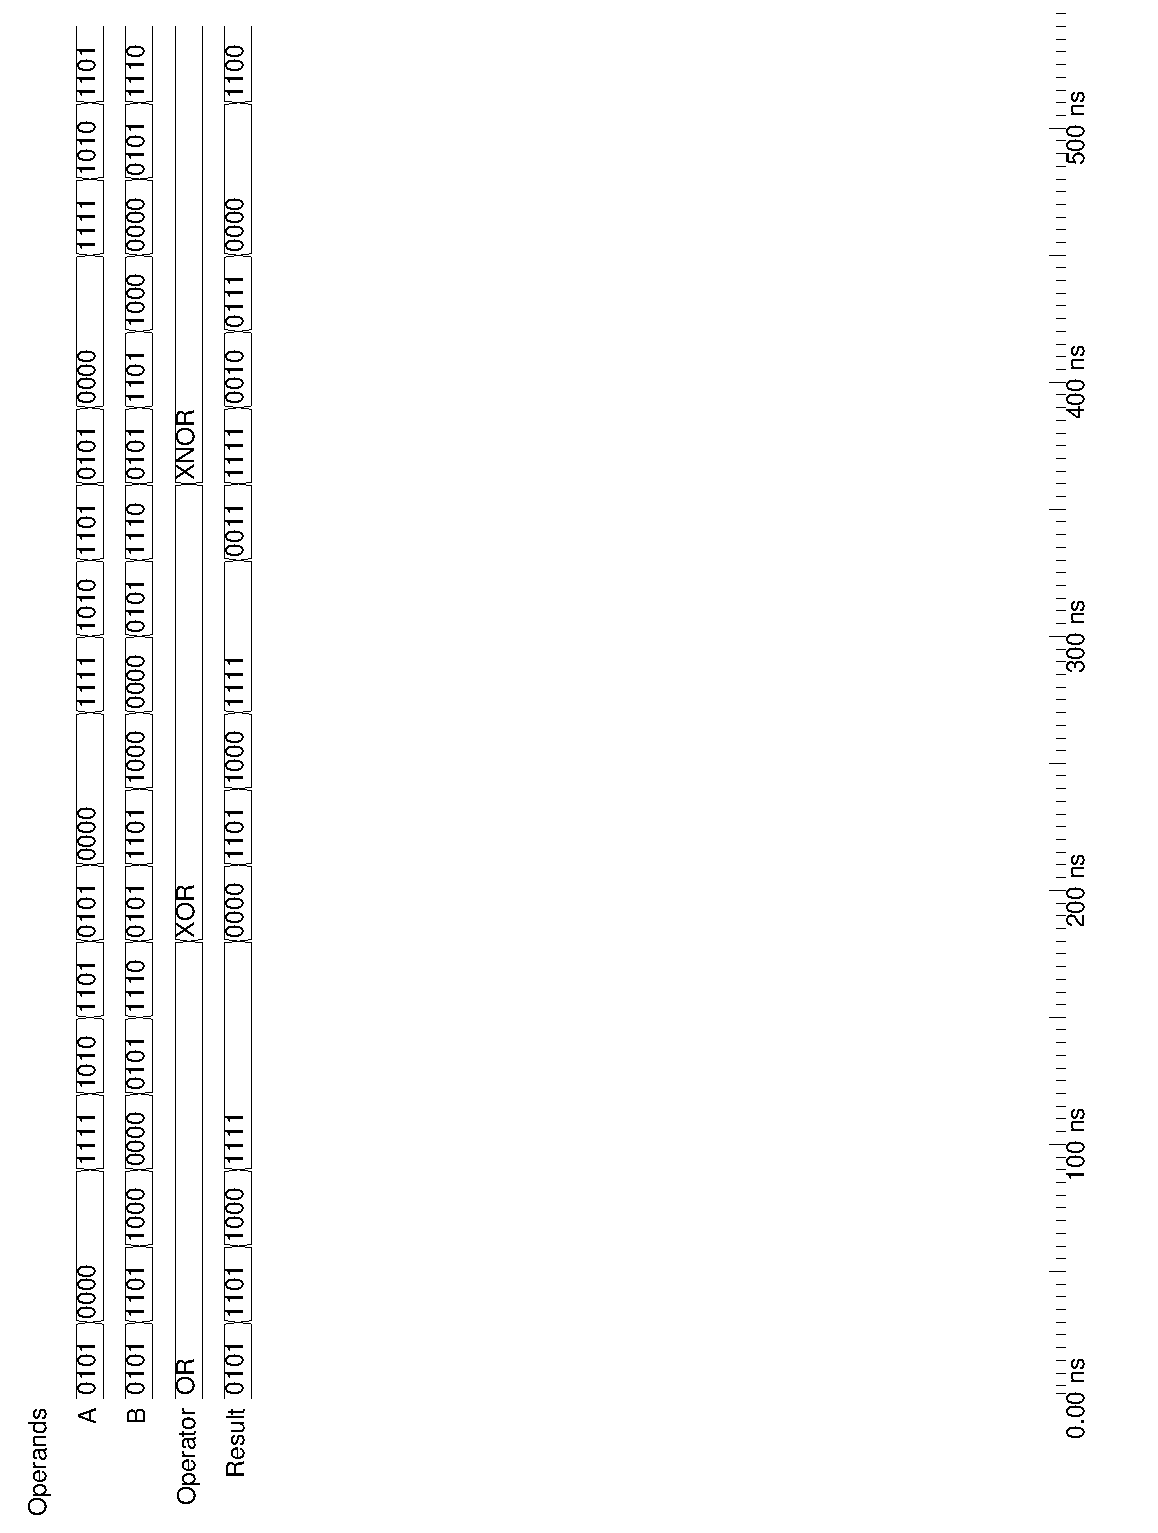
\includegraphics[scale=0.5,angle=-90]{graphs/alu_4bit_test2p1.ps}
\includegraphics[scale=0.5,angle=-90]{graphs/alu_4bit_test2p2.ps}
\caption{\small{Test result of logic operations}} \label{wave:alu:t2}
\end{figure}


 Figure \ref{wave:alu:t1} shows \texttt{for-loop} test
 in \emph{addition} and \emph{subtraction} modes. The
 overflow occurs at rather low values, proving that this
 ALU is not operational for arithmetics with result values
 greater then $+6$ or less then $-8$.

 Waveforms in figure \ref{wave:alu:t2} show the logic
 mode test results applying same input bit sequences.
 The testbench used a \texttt{for-loop} to cycle through
 the operator commands. The results were manually checked
 and found to be correct.

 \subsubsection{Conclusion}

 A 4-bit ALU without a carry output is rather unusable
 for arithmetics. This design would be useful as a building
 block to produce 8-, 12-, 16-, 24-bit and greater width
 units. However, there is no need for such component in VHDL,
 since only a minor modification to the ALU code  would be
 required to increase the capabilities. Thought, it is not
 as simple when hardware constraints are in place, because
 many different adder design pattern are available and the
 decision has to be made in terms of physical area, performance
 or power optimisation preferences made before loading the
 circuit design into programmable devices.

\begin{figure}
\includegraphics[scale=0.7]{graphs/alu_4bit.rtl.ps}
\caption{\small{RTL circuit diagram for ALU}} \label{rtl:alu}
\end{figure}
\pagebreak

\lstinputlisting[label=code:alu,
caption={\emph{Behavioural Implementation of 4-bit ALU}}]
{../code/comblogic/alu_4bit.listing.vhd}


\chapter{Design Units: Multifunctional Logic}

\section{Register}
\subsection{Description}

 Figure \ref{block:reg4} shows a block diagram with
 inputs and outputs of the register. \\ The opcodes for
 \texttt{Control} inputs are as fallows:

 \begin{tabular}{|c|c|l l|}
 \hline
 \texttt{Enable} & \texttt{Control}  & \emph{Command} & \emph{Function} \\
 \hline

 \texttt{0} & \texttt{XX} & \emph{HOLD} & $Q^{n+1} = Q^n$ \\

 \texttt{1} & \texttt{00} & \emph{CLEAR} & $Q^{n+1} = 0$ \\

 \texttt{1} & \texttt{11} & \emph{LOAD} & $Q^{n+1} = D^n$ \\

 \texttt{1} & \texttt{01} & \emph{OR BITS} & $Q^{n+1} = Q^n \cdot D^n$ \\

 \texttt{1} & \texttt{10} & \emph{AND BITS} & $Q^{n+1} = Q^n \oplus D^n$ \\

 \hline

 \end{tabular}

\begin{figure}
\center
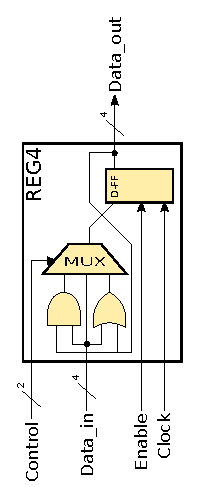
\includegraphics[scale=0.75,angle=-90]{graphs/reg_4bit.eps}
\caption{\small{Multifunctional register block diagram}} \label{block:reg4}
\end{figure}

\subsection{Verification}

 To simulate the register behaviour a simple testbench
 had been coded. The waveform in figure \ref{wave:reg4}
 demonstrates that changes in the output occur synchronously
 and the operation of this model does correspond to the given
 specification. 
 For example, the output doesn't clear until \texttt{Enable}
 input goes \emph{\texttt{high}} disregarding the state of
 \texttt{Control} input, also the output transaction doesn't
 occur until the rising edge of the \texttt{Clock} signal.
 Logic operations are also correct and synchronous.
 The RTL diagram (figure \ref{rtl:reg4}) appears to be
 very linear, nevertheless during HDL design of this model
 there had been a few errors made when the RTL viewer
 came in handy.

\begin{figure}
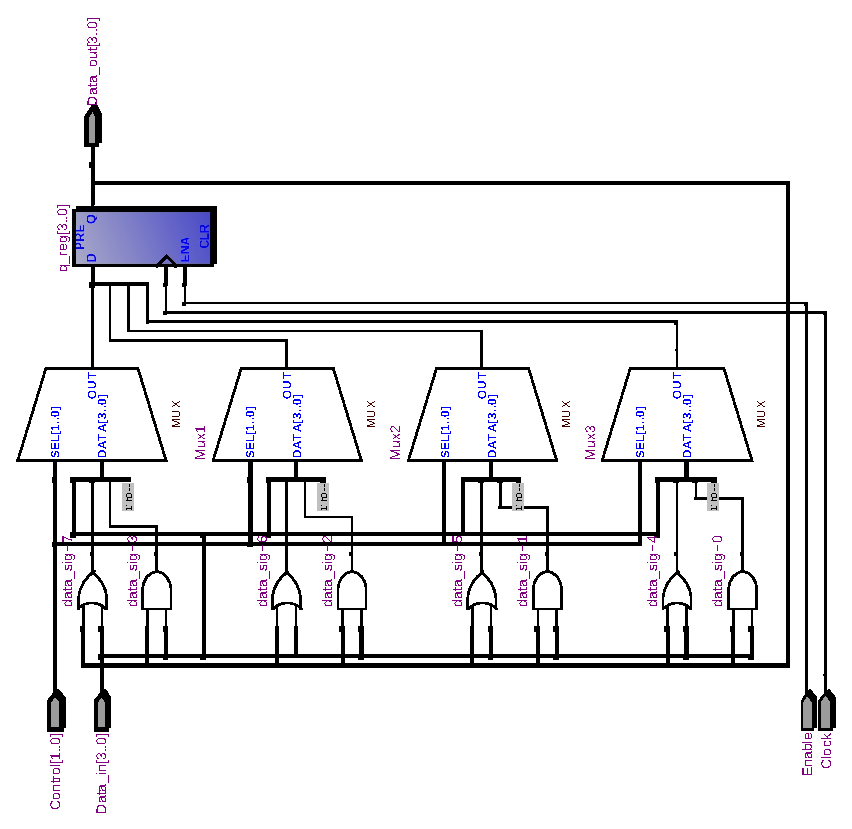
\includegraphics[scale=0.7,angle=-90]{graphs/reg_4bit.rtl.eps}
\caption{\small{Multifunctional register RTL circuit diagram}} \label{rtl:reg4}
\end{figure}

\begin{figure}
\center
\includegraphics[scale=0.4,angle=-90]{graphs/reg_4bit_test.ps}
\caption{\small{Multifunctional register simulation}} \label{wave:reg4}
\end{figure}

\pagebreak
\lstinputlisting[label=code:reg4,
caption={\emph{Behavioural Implementation of 4-bit register (brief)}}]
{../code/multifunc/reg_4bit.listing.vhd}

\pagebreak
\section{ENTITY}
\subsection{Description}

\subsection{Verification}

\pagebreak
\section{ENTITY}
\subsection{Description}

\subsection{Verification}

\end{document}
